% =====================================================================
% Problem statement. Rewritten to lead with the setting a practitioner has,
% then the one design choice that breaks, then the measured demonstration.
% Figure 1 block is preserved verbatim from the fig1_manifold rewrite.
% =====================================================================

\subsection{The setting: post-training a cloned policy}
\label{sec:setup}

A robot policy has been trained by behavior cloning on tens of
demonstrations, and it works, imperfectly. We want it to improve by
practising in its environment, with the only feedback being episode success.
Three features of this setting drive everything that follows:

\begin{itemize}
  \item \textbf{The demonstrations are few.} Whatever a learned critic knows,
  it learned from a thin shell of actions around them.
  \item \textbf{The reward is sparse.} A policy that stops succeeding
  receives a stream of zeros, which carries no information about how to
  succeed again.
  \item \textbf{The base policy is worth protecting.} It is the only thing in
  the system that reliably does the task at all.
\end{itemize}

Formally, states are $s$, actions are chunks $a \in \mathbb{R}^{H\times d}$ of
$H$ control steps flattened to dimension $S = Hd$, and reward is a sparse
task-success signal. The pretrained policy maps a state and a noise sample to
an action in a single network evaluation,
\begin{equation}
  a = \pi_0(s, z), \qquad z \sim \mathcal{N}(0, I),
\end{equation}
so the policy is a deterministic map from noise to action. Following standard
residual fine-tuning practice \citep{dawn2026,dicerl2026}, we freeze it and
learn a small residual on top,
\begin{equation}
  a = \pi_0(s,z) + r_\theta(s,z),
  \label{eq:residual}
\end{equation}
alongside an ensemble critic $Q_\phi(s,z,a)$ trained by temporal difference
with a conservative penalty \citep{kumar2020cql}. Critic training is identical
for every method we compare. \emph{The object of study is only the actor
update} --- how the policy consumes the critic it is given.

\subsection{Why the obvious tools do not apply}
\label{sec:failure-modes}

\paragraph{Policy gradients need a likelihood this policy does not have.}
PPO- and GRPO-style fine-tuners \citep{simplevlarl} require
$\log\pi(a\mid s)$. A one-step generator defines its action distribution
implicitly through the noise map, its likelihood is intractable, and unlike
multi-step diffusion there is no chain-MDP reformulation to fall back on
\citep{ren2024dppo,park2025fql}. Two routes recover a ratio and neither is
free. One \emph{changes the deployed policy}, adding Gaussian noise to its
output so a surrogate density exists \citep{reinflow2025}; we include it as a
baseline and it is competitive, but what ships is no longer the policy that
was pretrained. The other leaves the policy alone but requires it to \emph{be}
a flow model: FPO \citep{mcallister2025flowmatchingpolicygradients} builds a
clip ratio from differences of conditional flow-matching losses, which needs a
denoising loss over a flow time $\tau$ that a one-step model does not have. So
a critic is what remains, and the question becomes how to consume it.

\paragraph{Every critic-based update hands the critic two jobs.} A critic can
answer one question well: given this action, which way should it change to
score higher. Standard updates ask it a second question at the same time ---
how far --- and take the answer from the magnitude of its gradient.
Backpropagating $-Q$ through the actor, as in the DDPG lineage and DICE-RL's
residual actor \citep{dicerl2026}, does this explicitly,
\begin{equation}
  \nabla_\theta \mathbb{E}[-Q] = -\nabla_a Q \cdot \partial a/\partial\theta ,
  \label{eq:backprop-coupling}
\end{equation}
so a steeper critic produces a larger parameter step. The action-gradient
family \citep{dipo2024,psenka2024qsm} never differentiates through the policy,
but the improved action lands wherever $a + \alpha\nabla_a Q$ falls, so the
displacement is again proportional to the critic's steepness --- the same
delegation, one level up.

Only the first question is one the critic was trained to answer. It learns to
rank actions where it has data; away from that data nothing constrains it, and
it can be steep and wrong at once
\citep{fujimoto2018td3,fujimoto2019bcq,savo2025}. The two errors then fail
asymmetrically. A wrong \emph{direction} costs a slightly wrong step. A wrong
\emph{distance} costs the data manifold --- and once the policy is off it,
higher critic scores mean worse behavior, because the critic is scoring a
region it has never been corrected on.

One detail decides which remedy can work: the damage is \emph{persistent},
not sudden. The critic's extrapolated optimum does not recede as the policy
approaches it, so every update points the same way and nothing pulls the
policy back. A limit on step size therefore only slows the drift; a force
that returns the policy toward its starting point prevents it.
\Cref{sec:exp-constraint} measures both.

\subsection{Watching it happen}
\label{sec:toy}

We make the argument visible in a setting small enough to draw completely:
two-dimensional actions, a curved band of workable actions standing in for
the data manifold, and a reward that decays away from the band. A critic is
fit by regression to $25$ demonstrations sampled from the band --- only
demonstrated actions and their true rewards, exactly what a critic trained
on demonstration data sees.

\begin{figure}[t]
  \centering
  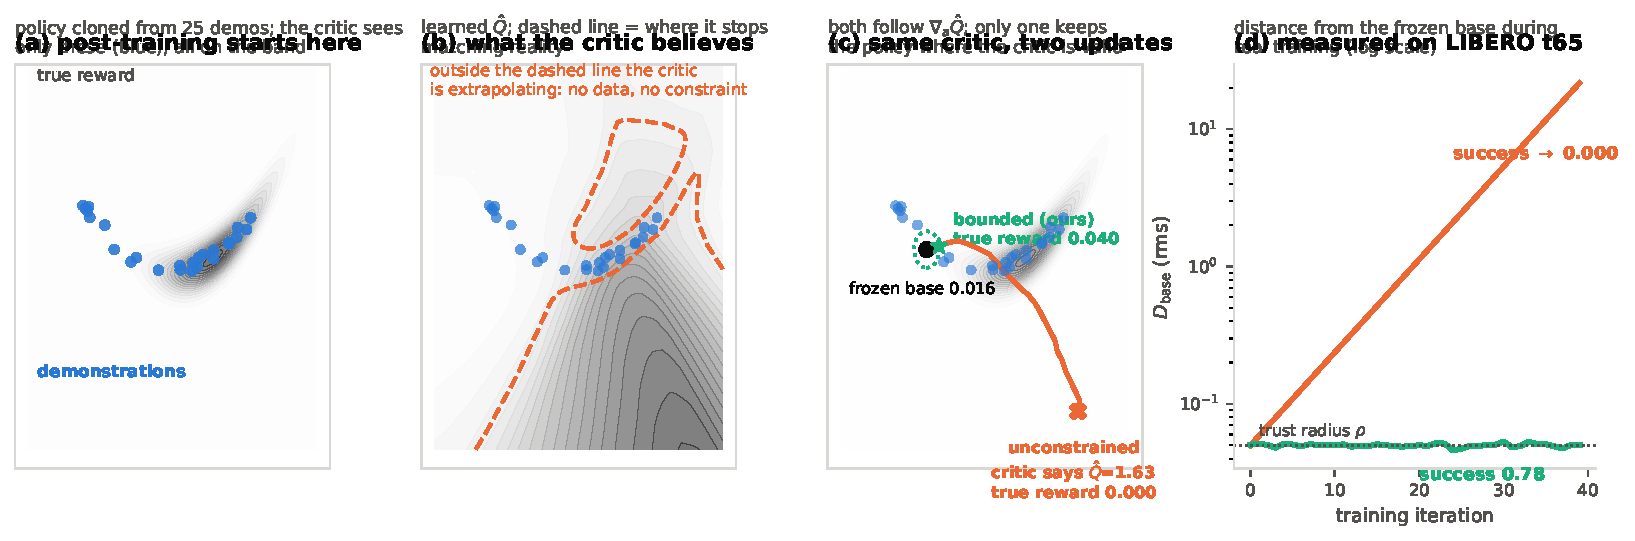
\includegraphics[width=\linewidth]{figures/fig1_manifold.pdf}
  \caption{\textbf{Why critic-guided post-training leaves the data, and what a
  bound does about it.} Panels (a)--(c) are computed, not drawn: a critic is
  fit by regression to $25$ demonstrations, the number a post-training setting
  actually has. \textbf{(a)} The task's true reward, and the demonstrations
  --- all of which lie on one narrow band of feasible actions. \textbf{(b)}
  What the critic learned. On the band it is accurate; beyond the dashed
  contour it has no data and is extrapolating, and nothing in its training
  penalises it for being confidently wrong there. \textbf{(c)} Two updates
  from the same start, both following $\nabla_a\hat{Q}$. The unconstrained one
  walks off the band to a point its own critic scores $\hat{Q}=1.63$ ---
  higher than \emph{any} achievable reward --- where the true reward is
  exactly $0.000$. Bounding the displacement around the frozen base keeps the
  policy where the critic is valid and improves it ($0.016\rightarrow0.040$,
  $2.5\times$). The gap between what the critic claims and what the policy
  earns is the whole failure. \textbf{(d)} The same mechanism in the
  real system: the residual norm logged during LIBERO red-mug training, from
  the runs behind \cref{tab:constraint}. Without a base-restoring term the
  residual immediately sits two orders of magnitude outside the dead zone and
  success is $0.000$; with it the residual stays an order of magnitude
  \emph{inside} the dead-zone radius --- the bound is slack, not binding ---
  and success is $0.600$.
  The regime matters: repeating (a)--(c) with $700$ demonstrations instead of
  $25$ removes the effect entirely (critic then learns the band and its
  gradient is trustworthy), which is why this paper scopes its claims to
  post-training from few demonstrations.}
  \label{fig:intuition}
\end{figure}
\Cref{fig:intuition}(a--c) shows the outcome: the critic is accurate on the
band and extrapolates freely beyond it, and following its gradient walks the
policy to a point scored $\hat{Q}=1.63$ --- above any achievable reward ---
where true reward is $0.000$, while the bounded update improves the same
start ($0.016 \rightarrow 0.040$). The effect has a data threshold, and that
threshold defines this paper's scope: at $200$ demonstrations the critic's
endpoint earns $0.901$ against its own estimate of $0.910$, so with enough
data the gradient is worth following without any bound. Critic gradients are
not untrustworthy in general --- only in the few-demonstration regime where
post-training happens, and every claim in this paper is scoped to it.

The same boundary can be crossed a second way, which rules out the objection
that our two-dimensional picture is a special case. Holding the amount of data
fixed and raising the \emph{dimension} of the action space shrinks the fraction
of that space the critic has seen, and produces the identical two regimes
(\cref{fig:toy}): with $2$-D actions the critic's gradient generalizes and
backpropagation is the best available update, while with $16$-D actions and the
same critic budget the same update drives true reward to zero as its internal
$Q$-estimate explodes. Coverage is the variable in both experiments; dimension
and demonstration count are two ways of changing it.

\begin{figure}[t]
  \centering
  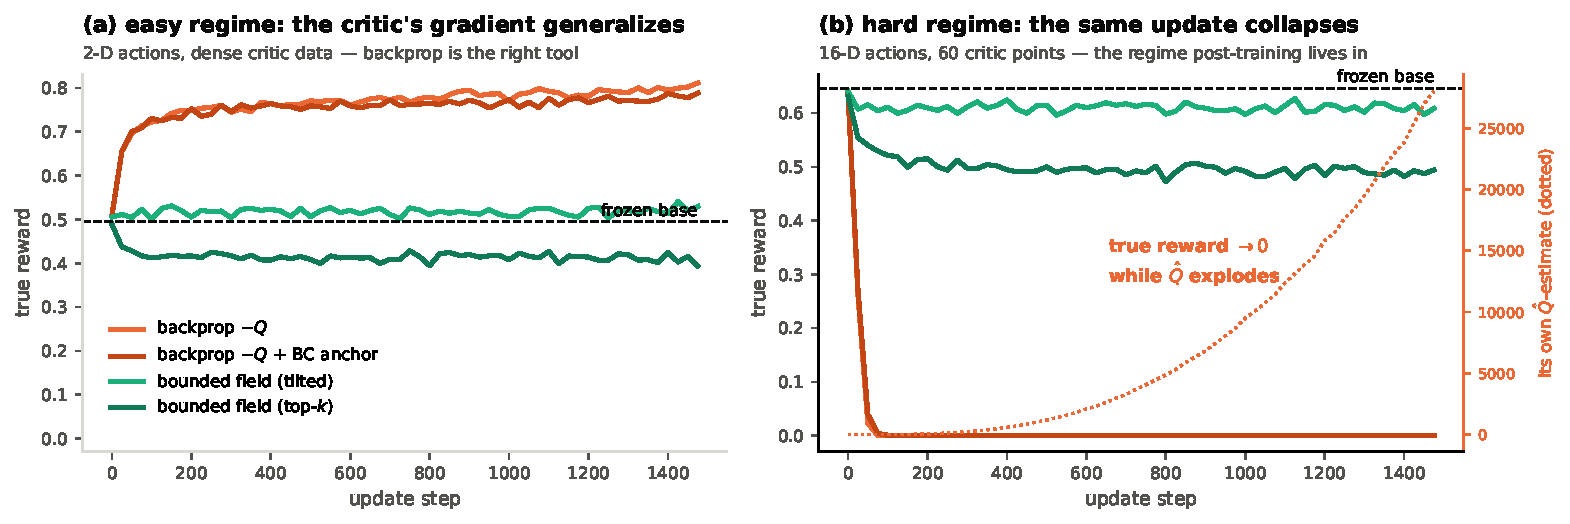
\includegraphics[width=\linewidth]{figures/toy_regimes.pdf}
  \caption{\textbf{The two-regime toy} (3-seed means). \textbf{(a) Easy
  regime} (2-D actions, dense critic data): the critic's gradient generalizes
  and backpropagating $-Q$ --- with or without a BC anchor --- is the best
  update, clearing both the base and the bounded field update.
  \textbf{(b) Hard regime} (16-D actions, 60 critic points, the coverage
  post-training actually has): the same updates drive true reward to zero
  within the first hundred steps, while the collapsing arm's \emph{own}
  $\hat{Q}$-estimate grows without bound (dotted, right axis) --- the critic
  rates the policy ever higher as it gets worse, and the BC anchor does not
  save it. The bounded field updates hold near the base throughout. A useful
  fine-tuner must exploit the gradient where it is trustworthy and survive
  where it is not.
  This sweeps the \emph{dimension} of the action space at fixed data, and
  \cref{fig:intuition} sweeps the \emph{amount} of data at fixed dimension;
  both cross the same boundary, which is what the critic's coverage of the
  region the update moves into.}
  \label{fig:toy}
\end{figure}
